\chapter{Methodology}\label{methodology}

\begin{figure}[t]
    \centering
    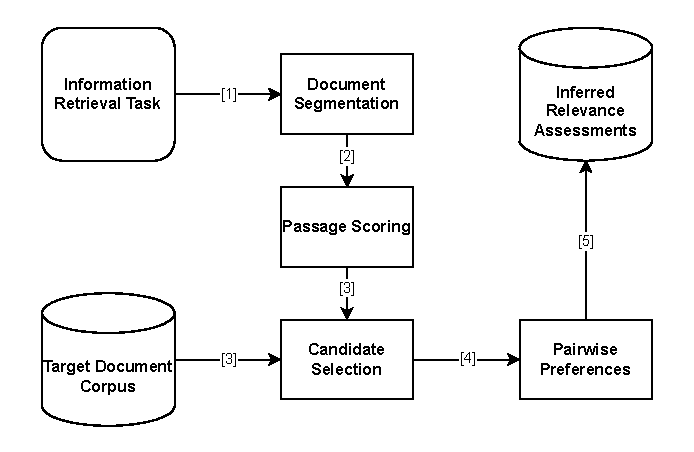
\includegraphics[width=\textwidth]{./graphics/drawio/transfer_pipeline.pdf}
    \caption{General overview of the transfer pipeline and its individual steps to transfer exisiting relevance assessments into another document corpus.}
    \label{fig:transfer-pipeline}
\end{figure}

In this Chapter, I present the individual steps of the transfer pipeline used for relevance transfer. The process begins with an information retrieval task consisting of a document corpus, a set of queries, and corresponding relevance judgments (Figure~\ref{fig:datasets}). The goal of the pipeline is to transfer the existing relevance judgments from a retrieval task to a target document corpus, thereby generating new relevance judgments. A simplified overview of the process is shown in Figure \ref{fig:transfer-pipeline}, which will now be explained in detail.
\\\\
The first step in the transfer pipeline involves selecting and segmenting documents from the retrieval task's document corpus. Only documents that contain at least one relevance judgment are selected, as those without any judgment do not provide useful information for the transfer process. Once selected, these documents are segmented into passages. This segmentation is done because relevant information related to an information need is typically concentrated in specific sections rather than spread across the entire document. By breaking documents into passages, the focus remains on the most relevant content. Additionally, since later stages of the pipeline rely on large language models, limiting the size of processed text through segmentation helps prevent potential issues when handling long documents with transformer models.
\\\\
The second step focuses on identifying the most relevant passages within each selected document. Therefore, the relevance of each passage is determined in respect to the query of its documents relevance judgment. To achieve this, each passage is treated as an independent query and submitted to the source document corpus. The resulting document rankings are then used to compute various evaluation metrics, which are assigned as passage scores. These scores are later used for selecting candidate documents from the target document corpus and identifying source passages for pairwise preference comparisons.
\\\\
The third step is the selection of candidate documents from the target document corpus. For each query in a retrieval task, a set of documents is chosen to receive new relevance judgments. This selection is performed using different strategies with the aim to identify documents most likely to be relevant. Each selected target document is then paired with relevant passages from the source dataset, identified in the previous step. These candidates serve as input for the pairwise inference process in the next step.
\\\\
At this stage, the transfer pipeline has identified, for each query, a set of target documents along with a corresponding set of relevant passages from the source dataset. The final step is inferring new relevance judgments for the target documents. To achieve this, target documents are also segmented into passages to be processed with source passages. Each query is then processed alongside a target passage and a source passage using a pairwise ranking model to determine whether the target passage is as relevant as the source passage. Finally, a label for an entire document from the target document corpus is then created by aggregating the relevance scores of all its passages.

% ========
% Datasets
% ========
\section{Datasets}\label{datasets}

\begin{table}[t]
    \centering
    \footnotesize
    \caption{List of source datasets and their associated retrieval tasks from which existing \texttt{qrels} where transferd into the target document corpus \texttt{ClueWeb22/b}.}
    \label{tab:datasets}
    \begin{tabular}{crcrrr}
        \toprule
        \multicolumn{2}{c}{\textbf{Corpus}} & \multicolumn{4}{c}{\textbf{ Associated Retrieval Tasks}} \\
        \cmidrule(lr){1-2} \cmidrule(lr){3-6}
        Name & documents  & Name & Queries &\texttt{qrels} & Labels \\
        \toprule
        
        Args.me & 0.4~m & Touché 2020 Task 1 & 49 & 2,298 & 3 \\
        \midrule

        \multirow{3}{*}{Disks4+5} & \multirow{3}{*}{0.5~m} & Robust04 & 250 & 311,410 & 3 \\
        & & TREC-7 & 50 & 80,345 & 2 \\
        & & TREC-8 & 50 & 86,830 & 2 \\
        \midrule

        \multirow{2}{*}{MS MARCO} & \multirow{2}{*}{3.2~m} & TREC 2019 DL Track & 43 & 16,258 & 4 \\
        & & TREC 2020 DL Track & 45 & 9,098 & 4 \\
        
        \bottomrule
    \end{tabular}
\end{table}

\begin{figure}[t]
    \centering
    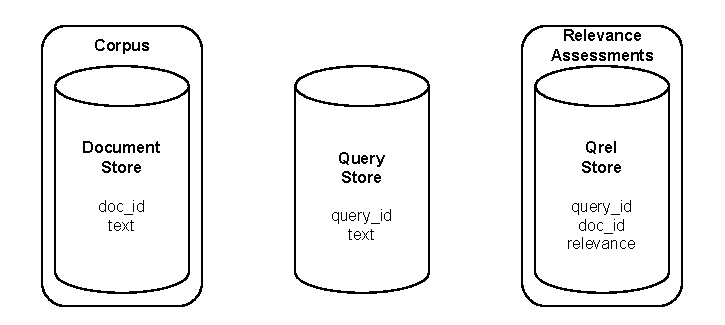
\includegraphics[width=\textwidth]{./graphics/drawio/datasets.pdf}
    \caption{Simplified structure of a dataset from \texttt{ir\_datasets}, comprising a set of documents, queries, and relevance judgments, along with their attributes.}
    \label{fig:datasets}
\end{figure}

Before the actual processing can begin, it is necessary to determine the source and target of the relevance transfer. This involves selecting datasets, along with their associated information retrieval tasks, as the foundation for transferring relevance judgments to a target document corpus.
\\\\
To simplify data handling, I used \texttt{ir\_datasets}~\citep{macavaney:2021}, a Python package that provides access to numerous information retrieval datasets. As illustrated in Figure~\ref{fig:datasets}, each dataset consists of a document corpus, a query \makebox[\textwidth][s]{store, and a set of relevance judgments for the queries and documents.}
\\\\\\
A key advantage of \texttt{ir\_datasets} is its standardized interface, which enables uniform access to different datasets. Through built-in iterators, the package facilitates structured access to corpora, queries, and relevance judgments, allowing the transfer pipeline to handle diverse datasets efficiently.
\\\\
The datasets and associated information retrieval tasks used in this thesis are listed in Table~\ref{tab:datasets}. The source datasets were selected based on their wide use in information retrieval research and their varying sizes. \texttt{Args.me} and \texttt{Disks4+5} are relatively small corpora, whereas \texttt{MS MARCO} is significantly larger. Additionally, the number of existing relevance judgments in these datasets varies considerably. \texttt{Args.me} contains approximately 2,300 judgments, while the retrieval tasks associated with \texttt{MS MARCO} have several thousand. In contrast, the tasks of \texttt{Disks4+5} extend far beyond this, with one exceeding 300,000 judgments. This diversity in dataset size and relevance judgment density provides a robust test for the transfer process under different conditions.
\\\\
The selected datasets serve as the starting point of the pipeline, while the final target corpus for relevance transfer is \texttt{ClueWeb22/b}. This dataset was chosen because it is the newest ClueWeb corpus in the \texttt{Lemur Project}\footnote{https://lemurproject.org}. With over 1.0~billion documents, \texttt{ClueWeb22/b} is significantly large, but due to its recent release, it currently has a low number of relevance judgments. The objective of the transfer process is to enrich \texttt{ClueWeb22/b} by leveraging the existing relevance judgments from the source datasets, thereby enhancing its use cases for information retrieval research.
\pagebreak


% =====================
% Document Segmentation
% =====================
\section{Document Segmentation}\label{document-segmentation}

\begin{figure}[t]
    \centering
    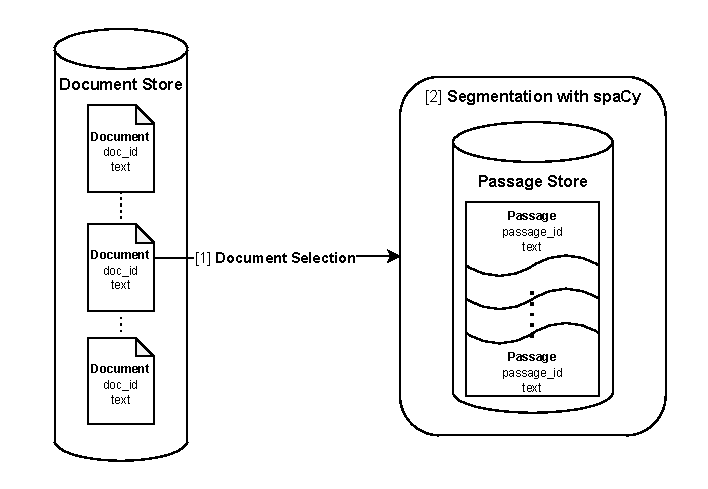
\includegraphics[width=\textwidth]{./graphics/drawio/document_segmentation.pdf}
    \caption{Visualization of the document segmentation step in the process pipeline. First, a subset of documents is selected from the document store. Then, the selected documents are segmented using \texttt{spaCy}.}
    \label{fig:document-segmentation}
\end{figure}

Now that the source datasets, along with their retrieval tasks and the target dataset, have been selected, the actual processing can begin. The first step in the transfer pipeline involves selecting and segmenting documents from the source dataset into passages as shown in Figure~\ref{fig:document-segmentation}. The primary objective is to transfer existing relevance judgments from the source retrieval task to the target corpus. This is done by using relevant documents, given through the existing relevance judgments, for each query in the retrieval task. These documents are the basis for comparison in the later pairwise preference step, alongside with documents from the target dataset. Because not all judged documents are required, only a representative subset is selected. The reason for this is that the later pairwise preferences require some comparison documents, but not all documents from the source document corpus. Additionally, this decreases the processing effort required for the transfer pipeline.Once the documents are chosen, they are segmented into passages, as relevance is often confined to specific sections rather than the entire document text. By breaking documents into passages, the pipeline can focus on the most relevant content while disregarding non-relevant parts of a document in the subsequent processing steps. Furthermore, later stages of the pipeline employ transformer models, which have a maximum input length they can process. Segmenting documents before passing them through LLMs ensures compliance with this constraint, allowing the models to work effectively \citep{levy:2024}.

% Document Selection
\subsection{Document Selection}\label{document-selection}

Instead of using the entire document corpus for relevance transfer, only a representative selection of documents is used, step [1] in Figure~\ref{fig:document-segmentation}. First, all documents without relevance judgments in the retrieval task can be ignored since they contain no useful information for the relevance transfer. Therefore, only judged documents are considered for selection. A document is considered judged if it has at least one relevance judgment in the \texttt{qrel store}. These judged documents, along with their relevance judgments for one or multiple queries of the retrieval task, can be used to transfer information, as their relevance has already been determined.
\\\\
The goal of this work is to transfer relevance judgments, which are assessments made by human annotators who assign relevance labels to documents based on a given query. As shown in Table~\ref{tab:datasets}, each retrieval task categorizes relevance judgments using different relevance labels. A relevance label specifies how relevant a document is to an information need, i.e., a query. This categorization varies in granularity. Some tasks use binary labels to distinguish only between relevant and non-relevant documents, while others employ a \mbox{Likert} scale to define multiple levels of relevance. In this thesis, no distinction is made between different levels of non-relevance, e.g., there is no differentiation between \glqq not relevant\grqq{} and \glqq strongly not relevant\grqq{}. This standardization was applied because finer distinctions among non-relevant documents were not deemed necessary for the research objectives.
\\\\
At this stage, all documents with at least one relevance judgment for any query of the retrieval task have been identified. Some retrieval tasks, such as \texttt{Robust04} with over 300,000 relevance judgments, contain a large number of judgments per query. As previously mentioned, only a representative subset of judged documents for each query is used for relevance transfer. To limit the number of judged documents in the transfer process, a maximum of 50 relevance judgments per relevance label of a retrieval task for each query, reffered to as query-label combination, is selected.
\\\\
Additionally, the number of documents for each query-label combination is capped at the minimum number of judged documents across all possible labels for that query. For example, if query $q$ has relevance judgments with label $0$, $1$, and $2$, and there are 30 relevance judgments with label $0$, 40 with label $1$, and 60 with label $2$, then 30 relevance judgments are selected for each of the three labels. This prevents bias toward labels with a higher number of judgments, ensuring a balanced representation of relevance labels within a query.

% Segmentation with spaCy
\subsection{Segmentation with spaCy}\label{segmentation-with-spacy}

Now that the documents used for relevance transfer have been selected, they are segmented into passages. This segmentation is performed to focus only on the most relevant parts of a document rather than the entire text and to ensure proper processing of text snippets through LLMs later. To achieve accurate segmentation with correct sentence separation, the GitHub repository \texttt{grill-lab/trec-cast-tools}\footnote{https://github.com/grill-lab/trec-cast-tools} was utilized. This repository provides a collection of scripts designed to process TREC CAsT Tracks \textcolor{red}{CITEP}. Among its features is the ability to process a document collection and generate passage splits.
\\\\
\texttt{trec-cast-tools} leverages \texttt{spaCy}\footnote{https://spacy.io}, a powerful natural language processing library in Python. \texttt{spaCy} offers various features, including tokenization, part-of-speech (POS) tagging, named entity recognition (NER), and lemmatization. It also provides functionality for sentence segmentation, which is used by \texttt{trec-cast-tools}. First, the documents are processed by \texttt{spaCy}, splitting the texts into sentences. Then, \texttt{trec-cast-tools} concatenates these sentences into passages, with each passage limited to a maximum length of 250 words.
\\\\
The selected documents from the source corpus are now available as uniquely identifiable passages, ensuring traceability throughout the transfer pipeline, which are saved in the \texttt{passage store}, see [2] Figure~\ref{fig:document-segmentation}. In cases where a document is judged as relevant to a query, the relevant information is often dispersed throughout the text. Therefore, in the next stage of the transfer pipeline, these individual passages are classified to identify those passages with a high density of relevant information. This step optimizes the results of the subsequent candidate selection and enhances the effectiveness of the pairwise preference process at the end of the pipeline.
\pagebreak


% ===============
% Passage Scoring
% ===============
\section{Passage Scoring}\label{passage-scoring}

\begin{figure}[t]
    \centering
    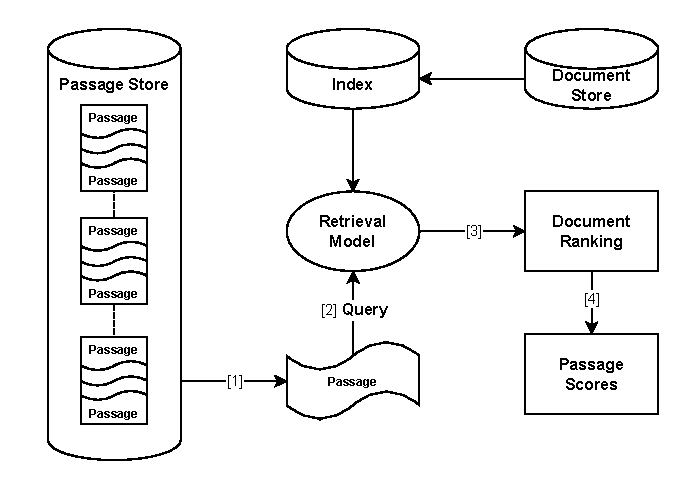
\includegraphics[width=\textwidth]{./graphics/drawio/passage_scoring.pdf}
    \caption{Generalised visualisation of the passage scoring process by submitting a passage as a query and retrieving a document ranking from the source corpus.}
    \label{fig:passage-scoring}
\end{figure}

As selected in Section \ref{document-selection}, each query-label combination of a retrieval task has an associated set of relevance judgments. To determine which passages of a document are most relevant and best reflect the label of its relevance judgment, a ranking of the individual passages is performed in this step. To rank all passages of the selected documents, the following procedure is applied to each relevance judgment which contains a selected document. First, each passage of a document is treated as an independent query, as shown in step [1, 2] Figure~\ref{fig:passage-scoring}. This query is then used to retrieve a document ranking from its original source \texttt{document store}, as shown in [3] Figure~\ref{fig:passage-scoring}. Based on the retrieved document ranking for the submitted passage, the relevance of the passage is determined by computing its \texttt{precision@10} and \texttt{nDCG@10} scores, step [4] Figure~\ref{fig:passage-scoring}. These metrics were chosen because they are widely used in information retrieval research. Additionally, \texttt{nDCG} provides a more fine-grained evaluation by considering relevance labels of the retrieved documents, whereas \texttt{precision} only accounts for binary relevance.
\\\\
\textbf{Precision} measures the fraction of retrieved documents that are relevant to a information need. In this context, the requested information is the original query associated with the relevance judgment to which the document of a passage belongs. A retrieved document is considered relevant if it has been judged as such in the relevance judgments of the retrieval task. To simplify passage scoring, the evaluation is restricted to the top 10 retrieved documents. The resulting \texttt{precision@10} score is then assigned as the ranking for the passage. This ranking represents the passage's relevance to the query of its original relevance judgment of the document it belongs to.
\\\\
\textbf{Normalized Discounted Cumulative Gain} (\texttt{nDCG}) is another metric commonly used in information retrieval to evaluate the quality of a ranking. Cumulative Gain (\texttt{CG}) represents the sum of all relevance labels for the retrieved document ranking. Again, the query of the retrieval task to which the document is assigned serves for determining the labels of the retrieved documents. Unlike \texttt{precision}, \texttt{CG} considers the label values instead of simply differentiating between non-relevant and relevant labels. This provides greater granularity in retrieval tasks with more than two labels, enabling more nuanced scoring of the passages of a document. The advanced Discounted Cumulative Gain (\texttt{DCG}) further refines this evaluation. It introduces a positional factor to the ranking. It assigns higher weight to relevant results that appear earlier in the ranking. The final score, \texttt{nDCG}, is calculated by normalizing the \texttt{DCG} score with the \texttt{Ideal DCG} (\texttt{IDCG}), which represents the optimal theoretical ranking for the query. As for \texttt{precision}, the evaluation is limited to the first 10 documents by calculating \texttt{nDCG@10}.
\\\\
The idea behind ranking document passages is that passages containing a high density of relevant information to an information need (i.e., the original query of a relevance judgment) are more likely to retrieve relevant documents and therefore achieve higher \texttt{precision@10} and \texttt{nDCG@10} scores. Conversely, passages with minimal or no relevant information will lead to lower scores due to fewer retrieved relevant documents.
\\\\
At this stage of the pipeline, the individual passages of the selected documents have been scored. These scores will serve as the foundation for the subsequent steps in identifying candidate documents from the target corpora. The selected candidates will receive newly inferred relevance judgments at the end of the pipeline. Additionally, these scores will help determine the most relevant passages from the source corpora, which will be used in pairwise preference comparisons alongside the selected candidates.


% ====================
% Candidate Retreiaval
% ====================
\section{Candidate Selection}\label{candidate-selection}

\begin{figure}[t]
    \centering
    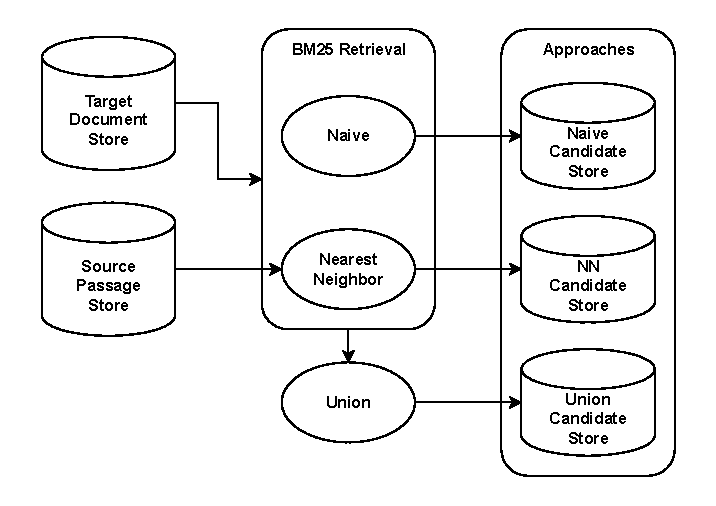
\includegraphics[width=\textwidth]{./graphics/drawio/candidate_selection.pdf}
    \caption{Tested approaches for the selection of documents from the target corpus for which relevance labels are to be determined.}
\end{figure}

The next step in the transfer pipeline is selecting candidates for pairwise preference inference at the end of the pipeline. This step consists of two parts. First, for each query in a retrieval task, documents from the target corpus are selected. New relevance judgments will be created for these queries and selected documents. The second part involves choosing passages from the source corpus for each query. These passages will be used in pairwise preference inference to determine whether a document from the target corpus is relevant to a given query.

% Document Retrieval from Target Dataset
\subsection{Document Retrieval from Target Dataset}\label{document-retrieval-from-target-dataset}

For each query in a retrieval task from the source dataset, a set of documents from the target corpus must be selected for which new relevance labels will be inferred. The goal is to identify documents that are most likely relevant to a query. By pre-selecting potentially relevant documents, the number of identified relevant documents at the end of the pipeline can be increased.
\\\\
To achieve this, all three tested approaches for selecting target documents begin with \texttt{BM25} retrieval as a pre-selection method. By submitting texts or passages, that are already identified as relevant for a query, against the target document store, a ranking of target documents is retrieved. The highest-ranked documents are the most likely to be relevant and therefore qualify for relevance label assignment. A fine-grained classification of relevance is performed later through pairwise preference inference. \texttt{BM25} retrieval was chosen for its efficiency \textcolor{red}{REF?} and because only an initial rough assessment is required.
\\\\
\textbf{Naive} The first approach, termed \texttt{naive}, submits each original query text from a retrieval task to the target corpus to retrieve potentially relevant documents. From the resulting document ranking, the top 1000 documents are selected as candidates. Unfortunately, some queries may be ambiguous, leading to multiple possible interpretations. For example, the query \glqq Apple\grqq{} could refer to either the technology company or the fruit. To address such ambiguities, the query description is also submitted as an independent query. A query description is a brief text that provides additional context, clarifying the search intent and specifying a query's focus. This retrieves another 1000 documents via \texttt{BM25} ranking. After filtering out duplicates between the two sets, up to 2000 unique documents per query are selected.
\\\\
\textbf{Nearest Neighbor} The second approach, \texttt{nearest neighbor}, is based on the relevant passages identified in Section~\nameref{passage-scoring}. In thies strategy, the top-scored passages for each query are submitted as queries to the target corpus. From the retrieved document ranking for each passage, the top 20 documents are selected as candidates for the corresponding query. As a result, each passage can contribute up to 20 unique documents to the candidate set.
\\\\
Several variations of the \texttt{nearest neighbor} were tested to determine the most effective candidate selection strategy. First, the number of selected top passages per query was limited. Three variations were evaluated: one using the top 10 passages, another using the top 50, and a third using the top 100 passages. This limitation significantly reduces the number of potential candidates, as a single query can have an exceedingly large number of relevant passages. The second variation introduced a restriction that allowed only one passage per original document to be used for retrieval, ensuring greater diversity in the selected candidates. In contrast, an alternative approach permitted multiple passages from the same document to be included. This variation was tested to assess the impact of passage diversity on retrieval effectiveness.
\\\\
\textbf{Union Approach} The third approach, called \texttt{union}, combines the \texttt{naive} and \texttt{nearest neighbor} approaches into a single candidate set for each query. This combination is intended to enhance the \texttt{Recall} of the number of retrieved relevant docuements by including a broader set of potentially relevant documents. However, the increased number of documents may reduce \texttt{Precision} by including more irrelevant entries, thereby increasing the workload for pairwise preference evaluations in later stages. The \texttt{Recall} and \texttt{Precision} of the approaches and variations are evaluated in Chapter~\ref{evaluation}~[\nameref{candidate-selection}].

% Postprocessing of Selected Target Documents
\subsection{Postprocessing of Selected Target Documents}\label{postprocessing-of-selected-target-documents}

As described in Section~\nameref{segmentation-with-spacy}, selected documents from the source dataset are segmented into passages for later processing. Since pairwise preferences will be applied at passage level, documents from both the source and target datasets have to be divided into passages. This is done using the same process as outlined before. First, \texttt{spaCy} is employed for segmenting the chosen target documents into sentences, and then passages are formed by concatenating sentences.

% Composing Final Candidates
\subsection{Composing Final Candidates}\label{composing-final-candidates}

For pairwise preference inference, a query, a passage from a document in the target corpus, and a known passage from the source corpus are needed (see \ref{fig:pairwise-preferences}). The queries are provided directly by the retrieval tasks. Now that the target documents have been identified, the selection of passages from the source dataset for pairwise preference inference can proceed. The goal is to compare each selected passage from the target corpus for a given query against 15 relevant and 5 non-relevant passages from the source corpus. To determine relevant and non-relevant passages, the computed passage scores from Section~\nameref{passage-scoring} are used.
\\\\
\textbf{Simple Selection} During the \nameref{passage-scoring} stage, each selected passage from the source corpus is evaluated and assigned scores based on the \texttt{precision@10} and \texttt{nDCG@10} metrics. These scores are now used to generate a ranking for each query. Following this strategy, the 15 highest-scoring passages and the 5 lowest-scoring passages for each query are selected.
\\\\\\\\\\\\\\\\
\textbf{Diversified Selection} It is possible that the top- and lowest-rated passages are predominantly drawn from a small subset of documents. While such passages may satisfy the selection criteria of the \texttt{simple selection}, this concentration could lead to unintended side effects by limiting variation in the pairwise preferences. To mitigate potential bias because of reduced document diversity, this approach restricts the selection to a maximum of one passage per document. Specifically, it selects the top 15 and bottom 5 passages for each query, ensuring that each passage is sourced from a distinct document. This strategy enhances diversity in pairwise preference comparisons by incorporating a wider range of source documents.
\\\\
For each query in a retrieval task, 20 selected passages, either from the simple or diversified selection approach, are chosen. These passages serve as a comparison standard in pairwise preference inference to determine the relevance of passages from the target corpus.
\pagebreak

% ====================
% Pairwise Preferences
% ====================
\section{Pairwise Preferences}\label{pairwise-transfering-relevance-labels-across-datasets}

\begin{figure}[t]
    \centering
    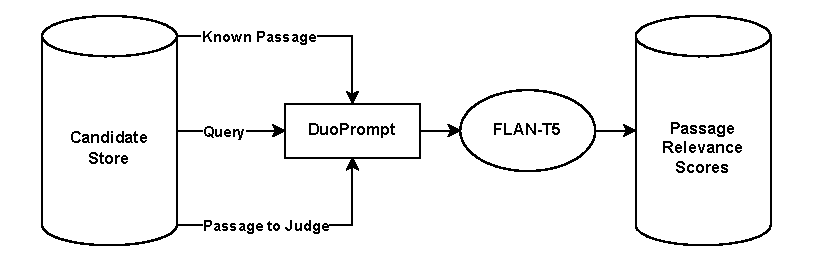
\includegraphics[width=\textwidth]{./graphics/drawio/pairwise_preferences.pdf}
    \caption{Visualization of the pairwise preference inference process with \texttt{DuoPrompt}. Each candidate consists of a query, a known passage from the source corpus, and a passage to judge from the target corpus.}
    \label{fig:pairwise-preferences}
\end{figure}

\begin{figure}[t]
    \centering
    \begin{tcolorbox}[title=One-Shot Prompt, width=\textwidth]
        \footnotesize
        \begin{verbatim}
PROMPT = (
    "Determine if passage B is as relevant as passage A "
    "for the given query. "
    'Passage A: "...{{ rel_doc_text | replace("\\"", "\'") }}..." '
    'Passage B: "...{{ unk_doc_text | replace("\\"", "\'") }}..." '
    'Query: "{{ query_text }}" '
    "Is passage B as relevant as passage A? </s>"
)
        \end{verbatim}
    \end{tcolorbox}
    \caption{One-shot prompt used for the \texttt{DuoPrompt} models in Figure~\ref{fig:pairwise-preferences}.}
    \label{fig:oneshot-prompt}
\end{figure}

So far, the transfer pipeline has selected a subset of documents from the source corpus for each query. These documents were then segmented into passages, and each passage was scored to identify the relevance of a passage, used for later processing steps. Subsequently, three approaches were described for determining candidates for pairwise preference inference. At this stage, all necessary processing steps have been completed to perform pairwise preference inference. As an output of Section \ref{candidate-selection}, each selected document from the target corpus has been broken down into passages and each passage is paired with 15 relevant and 5 non-relevant passages from the source corpus. The queries used for the pairwise preferences are predefined by the corresponding retrieval tasks. These resulting candidates, consisting of \texttt{(query, known passage, passage to judge)}, are now ready for processing, as visualized in Figure~\ref{fig:pairwise-preferences}.
\\\\
To perform the pairwise preference inference, the Python library \texttt{autoqrels}\footnote{https://github.com/seanmacavaney/autoqrels} was used. \texttt{autoqrels} is a tool designed for automatically inferring relevance judgments. It supports zero-shot and one-shot prompting for relevance inference and includes several pre-implemented inference models. The original \texttt{autoqrels} paper~\citep{macavaney:2023} evaluated the effectiveness of one-shot labelers for automatic relevance estimation. Among the tested approaches \texttt{MaxRep-BM25}, \texttt{MaxRep-TCT}, \texttt{DuoT5}, and \texttt{DuoPrompt}, the \texttt{DuoPrompt} approach for pairwise inference demonstrated superior performance and therefore was utilized for one-shot labeling in this thesis.
\\\\
\texttt{DuoPrompt} processes a $query$, a known passage $A$, and a passage to judge $B$. It constructs a prompt that includes a brief instruction before the query and passage texts, asking the model to assess the relevance of passage $B$ for the given query, as shown in Figure~\ref{fig:oneshot-prompt}. This prompt is then fed into \mbox{\texttt{FLAN-T5}~\citep{chung:2022}}, along with the question of whether passage $B$ is as relevant as passage $A$.
\\\\
\texttt{FLAN-T5} is a Text-to-Text Transfer Transformer model, an advanced version of Google's \texttt{T5} model~\citep{raffel:2020}. While maintaining the backbone architecture of \texttt{T5}, \texttt{FLAN-T5} has been further fine-tuned on a diverse set of training tasks, enhancing its performance across various natural language processing applications. \texttt{FLAN-T5} is available in multiple sizes, ranging from smaller, resource-efficient versions like \texttt{flan-t5-small}, with 80~million parameters, to larger models such as \texttt{flan-t5-xxl}, which contains 11~billion parameters. These variations accommodate different computational and application needs. Given the computational constraints for this thesis, \texttt{flan-t5-base} model \footnote{https://huggingface.co/google/flan-t5-base}, with 250~million parameters, was selected as the transformer model for \texttt{DuoPrompt}.
\\\\
Figure~\ref{fig:oneshot-prompt} illustrates the prompt structure provided to \texttt{FLAN-T5}. The prompt takes a query, a known passage (referred to as \texttt{rel\_doc\_text}), and a passage to judge (referred to as \texttt{unk\_doc\_text}) as inputs for pairwise inference. The model then predicts the probability values by computing the softmax over the logits of two tokens, which are subsequently used as the relevance score. If the passage to judge is highly relevant to the query, the model's expected output should be a score close to 1.0. Conversely, if the passage is not relevant, the model should produce a score close to 0.0.
\\\\
All candidates undergo pairwise preference inference, where each passage to judge is compared against 20 known passages, as outlined in Section \ref{composing-final-candidates}. Accordingly, the outcome of the pairwise preference inference generates 20 relevance scores for each passage to judge, with higher scores indicating greater relevance to the query. A final relevance for each query is then computed by aggregating all of its scores.
\\\\
This chapter has provided a comprehensive description of all steps in the transfer pipeline, resulting in a set of relevance scores for each passage to judge. These scores represent the transferred relevance judgments from the source dataset's retrieval task into the target corpus. The next chapter will evaluate the effectiveness of the individual steps and the overall quality of the transferred relevance judgments across datasets.